
\documentclass[a4paper]{article}
\usepackage[pdftex]{graphicx}
\usepackage[utf8]{inputenc}
\usepackage{enumerate}
\usepackage{siunitx}
\sisetup{locale=DE} 
\usepackage{icomma}
\usepackage{amssymb}
\usepackage{tikz}
\usepackage{href-ul}
\hypersetup{
	colorlinks=true,
	linkcolor=blue,
	urlcolor=blue}
\usepackage{geometry}
\geometry{a4paper, top=15mm, left=15mm, right=15mm, bottom=15mm,
	headsep=10mm, footskip=12mm}

\begin{document}
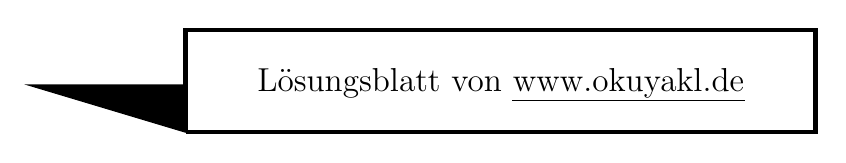
\begin{tikzpicture}(10,3)
	\draw[ultra thick](2,0) --(10,0) -- (10,1.3) --(2,1.3) -- (2,0);
	\draw[fill=black](2,0)-- (0,.6) -- (2,.6) -- (2,0);
	\node at (6,.6) {\large Lösungsblatt von \href{https://www.okuyakl.de}{www.okuyakl.de}};
\end{tikzpicture}
\vspace{0.5 cm}

\noindent
\begin{minipage}{0.4\textwidth}
\noindent{\bf Aufgabe 1. a)}\\
\includegraphics[width=7 cm]{della106}
\end{minipage}
\hfill
\begin{minipage}{0.6\textwidth}
\noindent{\bf Aufgabe 1. b)}\\
Die Längenausdehnungszahl errechnet sich mit:
$$\alpha = {\Delta l \over l_0 \cdot \Delta \vartheta}$$
\begin{tabular}{|cccc|}
	\hline
	$\vartheta$ in $\SI{}{\celsius}$ & 10 & 15 & 20 \\  
	$\Delta l$ in $\SI{}{\milli\meter}$ & 0,3 & 0,6 & 0,7 \\ 
	$\alpha$ in $\SI{}{\kelvin^{-1}}$& $3,0\cdot 10^{-5}$ & $4,0\cdot 10^{-5}$ & $3,5\cdot 10^{-5}$\\ 
	\hline
	$\vartheta$ in $\SI{}{\celsius}$ & 28 & 35 & 40\\
	$\Delta l$ in $\SI{}{\milli\meter}$ & 0,9 & 1,3 & 1,5 \\
	$\alpha$ in $\SI{}{\kelvin^{-1}}$ & $3,2\cdot 10^{-5}$ & $3,7\cdot 10^{-5}$ & $3,8\cdot 10^{-5}$\\
	\hline
\end{tabular}
\vspace{0.5 cm}

Der Mittelwert ist: $\alpha = \SI{3,5e-5}{\kelvin^{-1}}$
\end{minipage}
\vspace{0.5 cm}

\noindent {\bf Aufgabe 2.}\\
Es gilt für die Volumenzunahme des Benzins: 
$$\Delta V_B = V \cdot \gamma_{Benzin} \cdot \Delta \vartheta = 60~l \cdot 0,00106~{ 1 \over \SI{}{\celsius}} \cdot \SI{25}{\celsius} = 1,59~l$$
Der Tank nimmt ebenfalls an Fassungsvermögen zu:
$$\Delta V_T = V \cdot \gamma_{Stahl} \cdot \Delta \vartheta = 60~l \cdot 0,000036~{ 1 \over \SI{}{\celsius}} \cdot \SI{25}{\celsius} = 0,054~l$$
Die Menge des überlaufenden Benzins ist die Differenz hiervon:
$$V=\Delta V_B- \Delta V_T=1,54~l$$
\vspace{0.5 cm}

\noindent {\bf Aufgabe 3.}\\
Beim Eintauchen erwärmt sich zunächst der Glaskolben und wird dabei voluminöser. Die sich darin befindende, noch kalte Flüssigkeit weicht aus der Säule etwas zurück, bevor auch sie sich erwärmt und ausdehnt.
\vspace{0.5 cm}

\noindent {\bf Aufgabe 4. a)}\\
Das kühlere Wasser in Schenkel A ist nun schwerer als das übrige. Es sinkt nach unten, dann nach rechts. Oben strömt wärmeres Wasser von links nach. Es stellt sich im Rohrsystem eine Zirkulation gegen den Uhrzeigersinn ein.
\vspace{0.5 cm}

\noindent {\bf Aufgabe 4. b)}\\
Durch die Anomalie des Wassers ist es bei $\SI{4}{\celsius}$ am dichtesten. Es dehnt sich bei weiterer Abkühlung auf $\SI{1}{\celsius}$ wieder aus und wird folglich wieder leichter. Dies wirkt der Zirkulation entgegen; sie kommt zum Erliegen.
\vspace{0.5 cm}

\noindent {\bf Aufgabe 5. a)}\\
Das Gesetz von Gay-Lussac besagt, dass das Volumen eines idealen Gases proportional zu dessen Temperatur ist:\\
$V \sim T $ oder genauer 
$$ V = V_0\cdot (1+ {T \over \SI{273,15}{\kelvin}})\qquad (T ~in~\SI{}{\kelvin}) $$ 
Dies gilt nur, wenn der Druck konstant bleibt.
\vspace{0.5 cm}

\noindent {\bf Aufgabe 5. b)}\\
Nach dem Gesetz von Boyle-Mariotte ist der Druck eines idealen Gases umgekehrt proportional zum Volumen:
$$ p \sim {1 \over V} \quad \textnormal{oder} \quad p \cdot V = const.$$
Damit ist auch dieses Produkt proportional zur Temperatur. Wir verwenden als Konstante $R$:
$$ p \cdot V = R \cdot T $$ 
Dies ist die allgemeine Gasgleichung.
\vspace{0.5 cm}

\noindent {\bf Aufgabe 6.}\\
$$
\renewcommand{\arraystretch}{2}
\begin{array}{rcll}
{p_1 \cdot V_1 \over T_1} &=& {p_2 \cdot V_2 \over T_2} & |: p_2 \cdot T_2 \\
{p_1 \cdot V_1 \cdot T_2 \over p_2 \cdot T_1} &=& V_2 \\
V_2 &=& {\SI{1e5}{\pascal} \cdot \SI{1,2}{\meter^3} \cdot \SI{223}{\kelvin} \over \SI{264e2}{\pascal} \cdot \SI{291}{\kelvin}}\\
V_2 &=& \SI{3,5}{\meter^3} 
\end{array}
$$
\vspace{0.5 cm}

\noindent {\bf Aufgabe 7. a)}\\
Die Geschwindigkeit der Teilchen nimmt zu. $\Rightarrow$ Die kinetische Energie steigt.
Der Abstand der Teilchen zueinander verändert sich nicht $\Rightarrow$ Die potentielle Energie der Teilchen bleibt gleich.
\vspace{0.5 cm}

\noindent {\bf Aufgabe 7. a)}\\
Der Abstand der Teilchen zueinander nimmt zu. $\Rightarrow$ Die  potentielle Energie steigt. Die Geschwindigkeit der Teilchen verändert sich nicht $\Rightarrow$ Die kinetische Energie der Teilchen bleibt gleich.
\vspace{0.5 cm}


\begin{center}
	\includegraphics[width=7 cm]{../../viecher/endcomic.pdf}
	
	Hier geht es zurück zum \href{https://www.okuyakl.de/phys/p9thdL106/aa106.pdf}{Aufgabenblatt}
\end{center}

\end{document}